%===================================== CHAP 4 =================================

\chapter{Results and Analysis}
\label{chap:results}
Results are presented in the following chapter. The chapter is separated into sections in line with the categories defined in section~\ref{subsec:data-req}, in the following order: miscellaneous, research transparency, method documentation, experiment documentation,  and open data. Following these sections, researcher errors made during the evaluations is discussed. The chapter continues with an analysis of open source and open data in relation to author affiliation and conference instalment, ending with a look at methods and results reproducibility.

\section{Miscellaneous}
Variables in the miscellaneous category describe the research and include the following variables: affiliation, conference, research type, result outcome, and third-party citation.
The data for each variable except conference can be seen in figure~\ref{fig:miscellaneous-data}. The conference distribution is seen in table~\ref{tab:conferences}. There is a clear dominance of academia affiliated papers, amounting to 82.8\% (331) of the evaluated papers. Similarly, experimental papers dominate over theoretical, at 81.2\% (325).

Note that the Third-party citation data in figure~\ref{fig:third-party_citation} and Result outcome data in figure~\ref{fig:result_outcome} should not be used for analysis due to researcher error as discussed in section~\ref{sec:researcher_error}, but is presented for completeness.

\begin{table}[!h]
\begin{center}
    \begin{tabular}{ lr }
    \textbf{Conference} & \textbf{Papers} \\
    AAAI 14 & 100 \\
    AAAI 16 & 100 \\
    IJCAI 13 & 100 \\
    IJCAI 16 & 100 \\
    \end{tabular}
\end{center}
\caption{Distribution of papers between conferences.}
\label{tab:conferences}
\end{table}

\begin{figure}[!h]
\begin{center}
    \begin{subfigure}[b]{0.45\textwidth}
        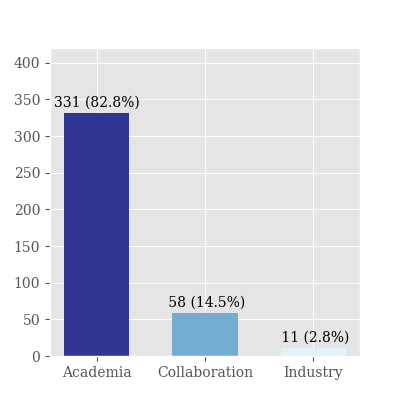
\includegraphics[width=\textwidth]{Affiliation.png}
        \caption{Affiliation}
        \label{fig:affiliation}
    \end{subfigure}
    \begin{subfigure}[b]{0.45\textwidth}
        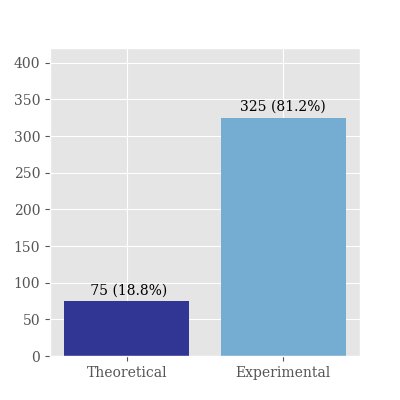
\includegraphics[width=\textwidth]{Research_Type.png}
        \caption{Research type}
        \label{fig:research_type}
    \end{subfigure}
    \begin{subfigure}[b]{0.45\textwidth}
        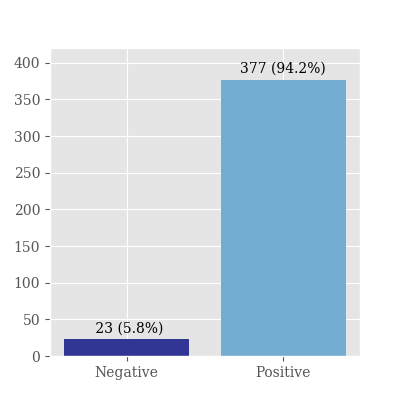
\includegraphics[width=\textwidth]{Result_Outcome.png}
        \caption{Result outcome}
        \label{fig:result_outcome}
    \end{subfigure}
    \begin{subfigure}[b]{0.45\textwidth}
        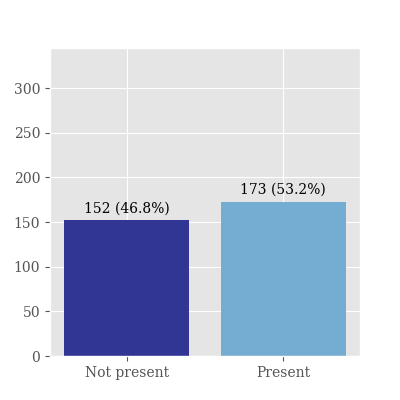
\includegraphics[width=\textwidth]{Third-party_Citation.png}
        \caption{Third-party citations}
        \label{fig:third-party_citation}
    \end{subfigure}
    \caption[Summary of miscellaneous data.]{Summary of miscellaneous data for all 400 papers. Note that for Third-party citation only the 325 experimental papers are relevant, which accounts for the lower values on the left axis.}
    \label{fig:miscellaneous-data}
\end{center}
\end{figure}
\clearpage

\section{Research Transparency}
Research transparency variables describe how well the research method is documented. This includes explicit mentions of: contribution, research goal or objective, hypothesis, prediction, problem description, research method, and research question. The distributions for each variable can be seen in figure~\ref{fig:transparency-data-a} and~\ref{fig:transparency-data-b}. The variables show little explicit mention the research background, with contribution (46.8\%), problem description (46.5\%), and goal/objective (20.2\%) mentioned most. The remaining variables are seen in between 1 and 5 percent of the papers. This indicates that few papers present their work in line with the scientific method as used by natural sciences, but may be influenced by the terms chosen and the strict requirement of explicit mentions.

\begin{figure}[!h]
\begin{center}
    \begin{subfigure}[b]{0.45\textwidth}
        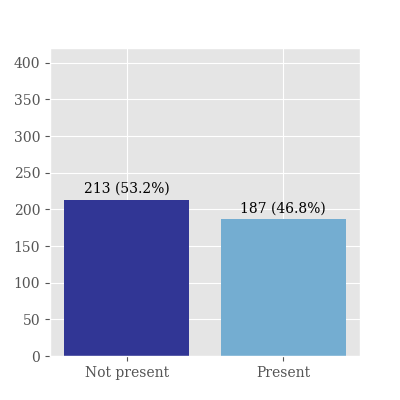
\includegraphics[width=\textwidth]{Contribution.png}
        \caption{Contribution}
        \label{fig:contribution}
    \end{subfigure}
    \begin{subfigure}[b]{0.45\textwidth}
        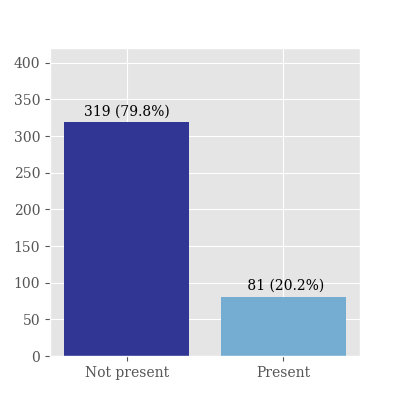
\includegraphics[width=\textwidth]{Goal_or_Objective.png}
        \caption{Goal or objective}
        \label{fig:goal_or_objective}
    \end{subfigure}
    \begin{subfigure}[b]{0.45\textwidth}
        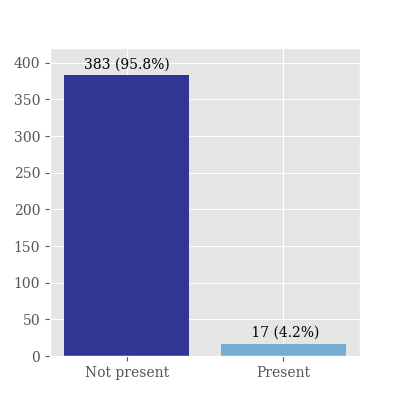
\includegraphics[width=\textwidth]{Hypothesis.png}
        \caption{Hypothesis}
        \label{fig:hypothesis}
    \end{subfigure}
    \begin{subfigure}[b]{0.45\textwidth}
        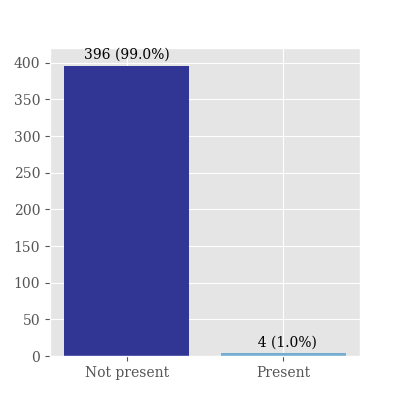
\includegraphics[width=\textwidth]{Prediction.png}
        \caption{Prediction}
        \label{fig:prediction}
    \end{subfigure}
    \caption[Summary of research transparency data.]{Summary of data on research transparency. A term is \emph{Present} if it is explicitly mentioned in a paper. These variables are applicable to all 400 papers.}
    \label{fig:transparency-data-a}
\end{center}
\end{figure}
\begin{figure}[!h]
\begin{center}
    \begin{subfigure}[b]{0.4\textwidth}
        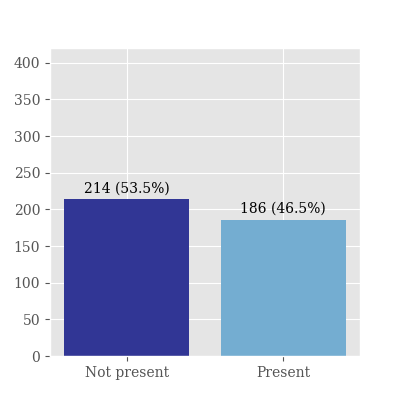
\includegraphics[width=\textwidth]{Problem_Description.png}
        \caption{Problem description}
        \label{fig:problem_description}
    \end{subfigure}
    \begin{subfigure}[b]{0.4\textwidth}
        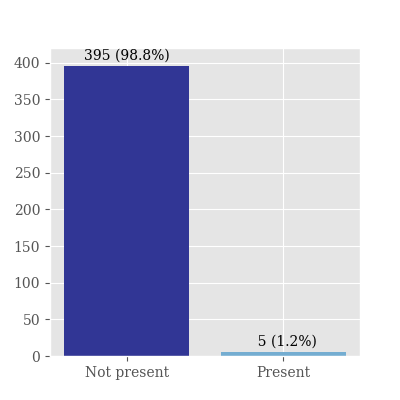
\includegraphics[width=\textwidth]{Research_Method.png}
        \caption{Research method}
        \label{fig:research_method}
    \end{subfigure}
    \begin{subfigure}[b]{0.4\textwidth}
        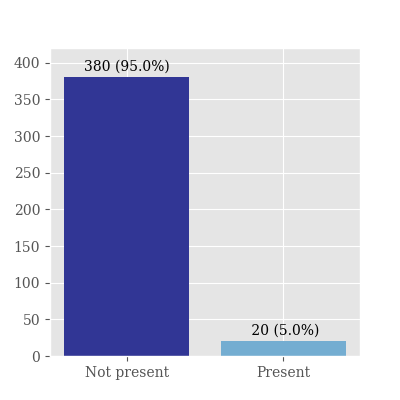
\includegraphics[width=\textwidth]{Research_Question.png}
        \caption{Research question}
        \label{fig:research_question}
    \end{subfigure}
    \caption[Summary of research transparency data continued.]{Continued summary of data on research transparency. A term is \emph{Present} if it is explicitly mentioned in a paper. These variables are applicable to all 400 papers.}
    \label{fig:transparency-data-b}
\end{center}
\end{figure}
\clearpage

\section{Method Documentation}
The method documentation category investigates the availability of the method under investigation through the pseudo-code, and open source code variables. Only the 325 experimental papers are relevant for these variables, as seen by the lower values on the left axis compared to the transparency data. The data is summarised in figure~\ref{fig:method_documentation}. Pseudo-code is present in about half (54.5\%) of the examined papers. The variable is not a good estimate for how many document their method, however, as there are other ways to present it. The papers without pseudo-code often include mathematical expressions to describe methods. Open source code is only seen in 26 (8\%) of the papers. A few papers reference material that was not found during the evaluation or that material will be published in the future.

\begin{figure}[!h]
\begin{center}
    \begin{subfigure}[b]{0.4\textwidth}
        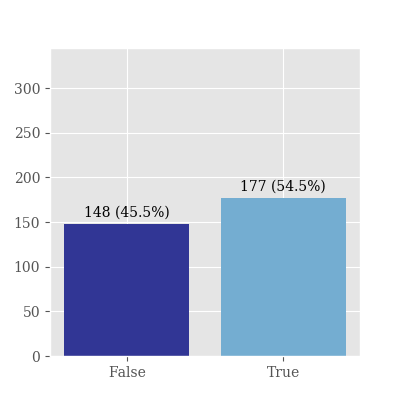
\includegraphics[width=\textwidth]{Pseudocode.png}
        \caption{Pseudo-code}
        \label{fig:pseudocode}
    \end{subfigure}
    \begin{subfigure}[b]{0.4\textwidth}
        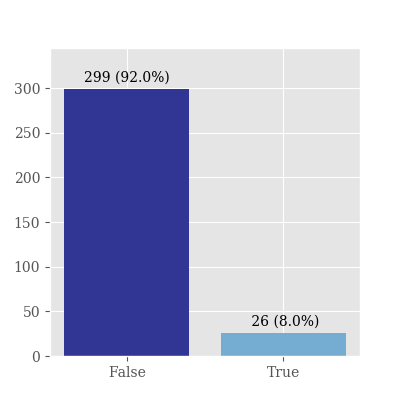
\includegraphics[width=\textwidth]{Open_Source_Code.png}
        \caption{Open source code}
        \label{fig:open_source_code}
    \end{subfigure}
    \caption[Summary of method documentation data.]{Summary of data for the method documentation category. These variables are only applicable to the 325 experimental research papers.}
    \label{fig:method_documentation}
\end{center}
\end{figure}

\section{Experiment Documentation}
Experiment documentation variables relate to how well the experiment is documented and if it is made available. The following variables are included: evaluation criteria, experiment set-up, hardware specification, open experiment code and software dependencies. A summary of the data can be seen in figure~\ref{fig:experiment_documentation}. As in the method documentation category, only the experimental papers are relevant. Open experiment code (5.5\%), hardware specification (27.4\%), and software dependencies (16.0\%) are the least documented variables on experiments. Sharing of experiment code is a little bit lower than sharing of source code (8\%). Evaluation criteria seems low at 47.1\%, but the evaluation was a little stricter than the procedure in section~\ref{sec:evaluation-procedure}, requiring explicit mentions of the criteria and not just shown as results. Experiment set-up is also covered in section~\ref{sec:researcher_error}, and covers papers that mention and discuss hyper-parameters rather than describing the necessities of how to conduct the experiment.

\begin{figure}[!h]
\begin{center}
    \begin{subfigure}[b]{0.4\textwidth}
        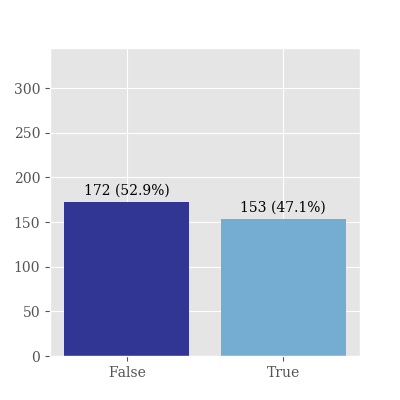
\includegraphics[width=\textwidth]{Evaluation_Criteria.png}
        \caption{Evaluation criteria}
        \label{fig:evaluation_criteria}
    \end{subfigure}
    \begin{subfigure}[b]{0.4\textwidth}
        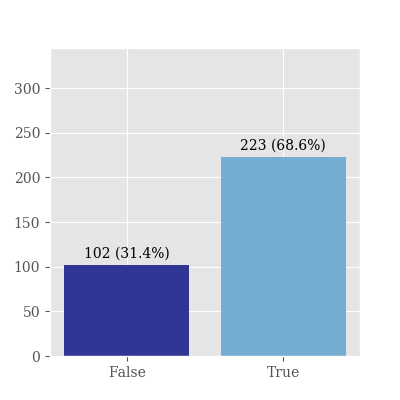
\includegraphics[width=\textwidth]{Experiment_Setup.png}
        \caption{Experiment set-up}
        \label{fig:experiment_setup}
    \end{subfigure}
    \begin{subfigure}[b]{0.4\textwidth}
        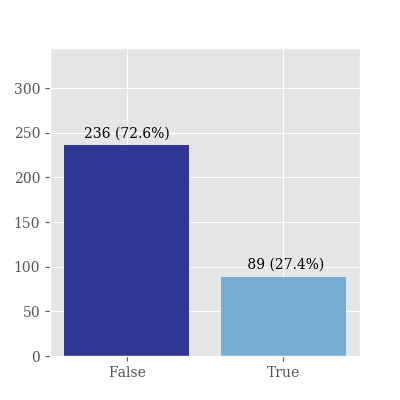
\includegraphics[width=\textwidth]{Hardware_Specification.png}
        \caption{Hardware specification}
        \label{fig:hardware_specification}
    \end{subfigure}
    \begin{subfigure}[b]{0.4\textwidth}
        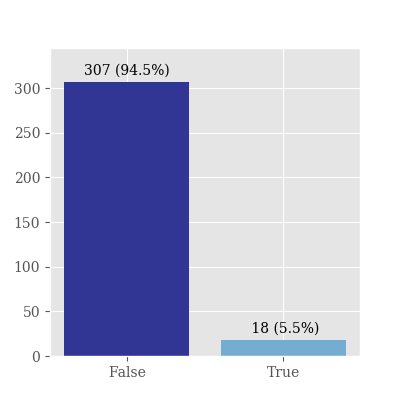
\includegraphics[width=\textwidth]{Open_Experiment_Code.png}
        \caption{Open experiment code}
        \label{fig:open_experiment_code}
    \end{subfigure}
    \begin{subfigure}[b]{0.4\textwidth}
        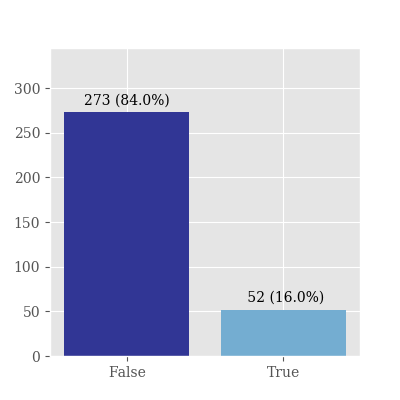
\includegraphics[width=\textwidth]{Software_Dependencies.png}
        \caption{Software dependencies}
        \label{fig:software_dependencies}
    \end{subfigure}
    \caption[Summary of experiment documentation data.]{Summary of data from the experiment documentation category. These variables are only applicable to the 325 experimental research papers.}
    \label{fig:experiment_documentation}
\end{center}
\end{figure}

\section{Open Data}
Open Data relates to the availability of data used during an experiment and documentation of dataset splits. The following variables are included: training data, validation data, test data, and results data. Figure~\ref{fig:open_data} summarizes the results for experimental papers. Most of the papers sharing open data do so indirectly by using public datasets, accounting for the higher proportion of training (32.0\%) and test data (29.8\%) compared to validation data (9.2\%). The amount of papers with open validation data would be closer to open training data if specifying the type of cross-validation used was not required. Results data is rarely shared (3.7\%), but occasionally bundled with the open source code.

\begin{figure}[!h]
\begin{center}
    \begin{subfigure}[b]{0.4\textwidth}
        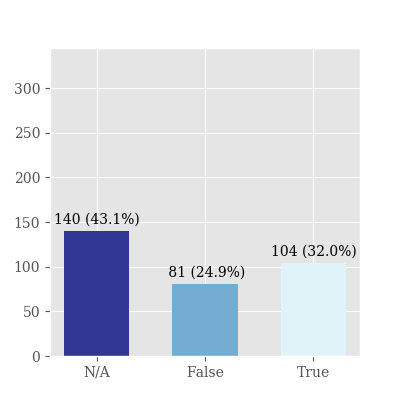
\includegraphics[width=\textwidth]{Training_Data.png}
        \caption{Open training data}
        \label{fig:training}
    \end{subfigure}
    \begin{subfigure}[b]{0.4\textwidth}
        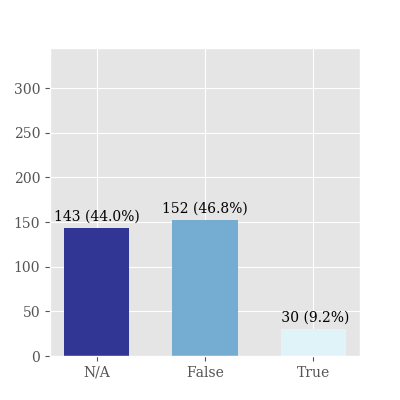
\includegraphics[width=\textwidth]{Validation_Data.png}
        \caption{Open validation data}
        \label{fig:validation}
    \end{subfigure}
    \begin{subfigure}[b]{0.4\textwidth}
        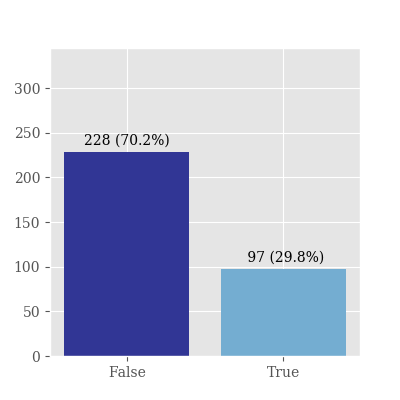
\includegraphics[width=\textwidth]{Test_Data.png}
        \caption{Open test data}
        \label{fig:test}
    \end{subfigure}
    \begin{subfigure}[b]{0.4\textwidth}
        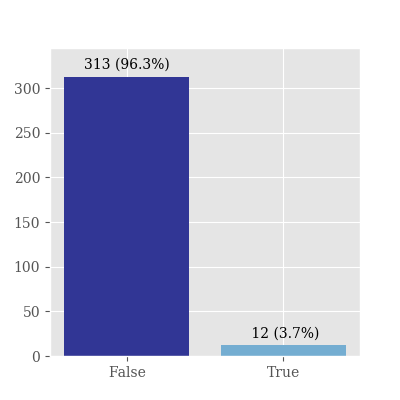
\includegraphics[width=\textwidth]{Results_Data.png}
        \caption{Open results data}
        \label{fig:results}
    \end{subfigure}
    \caption[Summary of the open data category.]{Summary of the open data category. These variables are only applicable to the 325 experimental research papers. Of special note is the \emph{N/A} column in (a) and (b), which shows the amount of papers where either training or validation data was deemed to not have been used in a paper due to the nature of the methods presented. This skews the percentage distribution. Percentages without \emph{N/A} amount to: (a) 43.8\% \emph{False} and 56.2\% \emph{True}, and (b) 83.5\% \emph{False} and 16.5\% \emph{True}.}
    \label{fig:open_data}
\end{center}
\end{figure}

\section{Researcher Error}
\label{sec:researcher_error}
The data for Third-party citations and Result outcome have been excluded from further analysis due to inaccurate data and researcher error, respectively. Experiment set-up divulged from the original intent, becoming a measure of whether parameters used to instantiate the method and experiment is mentioned or discussed rather than a description of the experiment.

For Third-party citations, the intent was to record citations of software and data used for an experiment. This intent was to investigate if public datasets and published source code is cited when used by other researchers. For the most part, the papers noted with \emph{Present} in figure~\ref{fig:third-party_citation} show correct citations to public datasets. However, it is difficult to say if a paper with a \emph{Not present} used third-party software or data at all, or failed to cite it properly.

Result outcome (figure~\ref{fig:result_outcome}) was erroneously recorded as a positive result, instead of a notion of the novelty of the research. This would be any paper that presents confirmation of a hypothesis, or where the wording of their findings present a solution or improvement to something. Since very few papers include a hypothesis in the first place, the data for this variable is excluded from any further analysis.
\clearpage

\section{Patterns of Analysis Revisited}
The patterns for analysis from \ref{subsec:data-req} were: (I) reproducibility in relation to author affiliation, (II) reproducibility related to conference and instalment year, and (III) reproducibility related to novelty of research. Since the result outcome variable for novelty of research was evaluated erroneously, data for this analysis is not presented. The variables investigated for these relations are all variables related to open source code or open data.

The differences in the variables open source code, experiment code, training, validation, test and results data when author affiliation is accounted for can be seen in table~\ref{tab:affiliation}. There is little to suggest significant impact on sharing from these data, keeping in mind that papers affiliated with academia amount to 265, collaboration to 50 and industry to 10. The industry sample size is too small to compare with the others, while the differences in collaboration and academia is small. The largest difference can be seen in open training data, academia at 61.0\% and collaboration at 45.7\%, potentially due to collaborations with industry giving academic researchers access to industry data not shared publicly. This has not been investigated further, however.

\begin{table}[!h]
\begin{center}
    \begin{tabular}{ r|cccc }
    \textbf{Variable} & \textbf{Academia} & \textbf{Collaboration} & \textbf{Industry} \\ \hline
    Open source code & 23 (8.7\%) & 2 (4.0\%) & 1 (10\%) \\
    Open experiment code & 15 (5.7\%) & 2 (4.0\%) & 1 (10\%) \\
    Open training data & 86 (61.0\%) & 16 (45.7\%) & 2 (22\%) \\
    Open validation data & 25 (17.9\%) & 5 (14.7\%) & 0 (0\%) \\
    Open test data & 80 (30.2\%) & 15 (30.0\%) & 2 (20\%) \\
    Open results data & 11 (4.2\%) & 0 (0\%) & 1 (10\%) \\
    \end{tabular}
\end{center}
\caption[Open source and data compared to affiliation.]{Differences in adoption of open source and data based on affiliation. It is important to note that the amount of experimental papers affiliated with academia dominates at 265, compared to 50 and 10 for collaboration and industry respectively For training data and validation data, some papers are N/A: respectively 124 and 125 for academia, 15 and 16 for collaboration, and 1 and 2 for industry.}
\label{tab:affiliation}
\end{table}

The split between conferences for experimental papers is as follows: 85 papers from AAAI 14, 85 papers from AAAI-16, 71 papers from IJCAI 13, and 84 papers from IJCAI 16. The high amount of papers not applicable to training and validation set from IJCAI 13 is likely due to the sample population involving 58 papers from the agent track, mentioned in section~\ref{sec:data-generation}. Considering the confidence intervals for the 100 paper sample sizes for each conference are just below 9\%, none of the variables in table~\ref{tab:pattern-conferences} have detectable differences between instalments, or differences between the 2013/14 instalments compared to 2016.

\begin{table}[!h]
\begin{center}
    \begin{tabular}{ r|cccc }
    \textbf{Variable} & \textbf{AAAI 14} & \textbf{AAAI 16} & \textbf{IJCAI 13} & \textbf{IJCAI 16}\\ \hline
    Open source code & 7 (8.2\%) & 9 (10.6\%) & 2 (2.8\%) & 8 (9.5\%) \\
    Open experiment code & 4 (4.7\%) & 6 (7.1\%) & 0 (0\%) & 8 (9.5\%) \\
    Open training data & 25 (51.0\%) & 39 (60\%) & 9 (42.8\%) & 31 (51.7\%) \\
    Open validation data & 5 (10.4\%) & 9 (13.8\%) & 4 (20.0\%) & 12 (20.3\%) \\
    Open test data & 24 (28.2\%) & 30 (35.3\%) & 13 (18.3\%) & 30 (35.7\%) \\
    Open results data & 2 (2.4\%) & 2 (2.4\%) & 0 (0\%) & 8 (9.5\%) \\
    \end{tabular}
\end{center}
\caption[Open source and data compared to conference instalment.]{Differences in adoption of open source and data based on conference instalment. The amount of experimental papers for each conference is as follows: 85 for AAAI 14, 85 for AAAI 16, 71 for IJCAI 13, and 84 for IJCAI 16. For training data and validation data, some papers are N/A: respectively 36 and 37 for AAAI 14, 20 and 20 for AAAI 16, 50 and 51 for IJCAI 13, and 34 and 35 for IJCAI 16.}
\label{tab:pattern-conferences}
\end{table}

\section{Reproducibility}
The importance of open source and data to methods and results reproducibility is shown in figure~\ref{fig:reproducibility}. For methods reproducibility, a paper is considered good enough if experiment and source code, as well as all data except results data is available. For results reproducibility, the data requirements are removed. As low as 3.1\% (10 papers) make both code and data available to allow methods reproduction. Papers covering the variables for results reproduction amount to 5.2\% (17 papers). Out of the 26 papers where the method source code is available, 17 of them include the experiment. Out of the 18 papers where the experiment code is available, 17 include the method code as well.

\begin{figure}[!h]
\begin{center}
    \begin{subfigure}[b]{0.4\textwidth}
        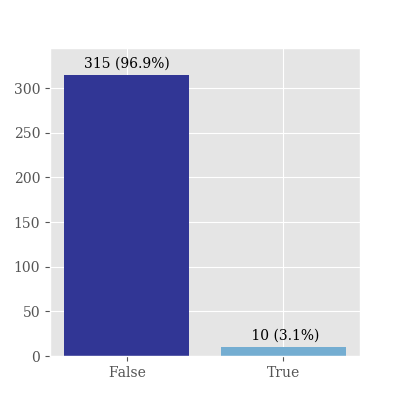
\includegraphics[width=\textwidth]{Methods_Reproducible.png}
        \caption{Methods reproducible papers}
        \label{fig:methods_reproducible}
    \end{subfigure}
    \begin{subfigure}[b]{0.4\textwidth}
        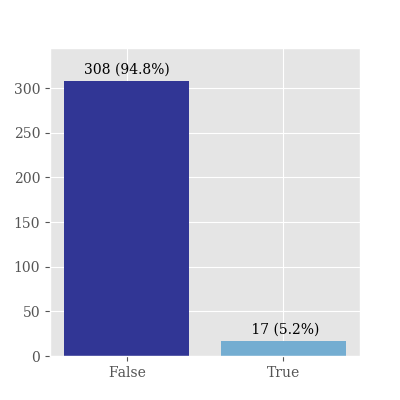
\includegraphics[width=\textwidth]{Results_Reproducible.png}
        \caption{Results reproducible papers}
        \label{fig:results_reproducible}
    \end{subfigure}
    \begin{subfigure}[b]{0.4\textwidth}
        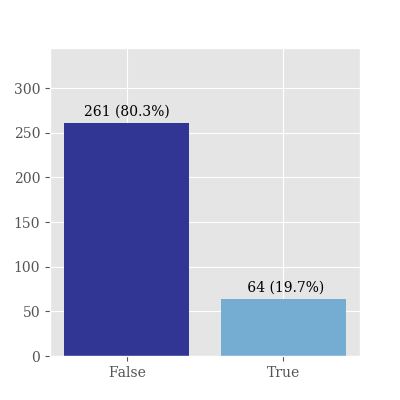
\includegraphics[width=\textwidth]{Data_Sets.png}
        \caption{Papers with open training, validation and test data sets.}
        \label{fig:data_sets}
    \end{subfigure}
    \caption[Amount of reproducible papers.]{The amount of experimental papers covering (a) methods and (b) results reproducibility as defined in \cite{Goodman341ps12}. (c) Shows the amount of papers where training, validation and test sets are available if applicable, highlighting a drop from 19.7\% with necessary data to 3.1\% with data and code for methods reproducible papers. Papers where training or validation set is not applicable are counted as True if the remaining variables are 1.}
    \label{fig:reproducibility}
\end{center}
\end{figure}

\cleardoublepage
